\section{Results}
\label{ch:results}
\noindent	

\begin{figure}[H]
	\begin{center}
		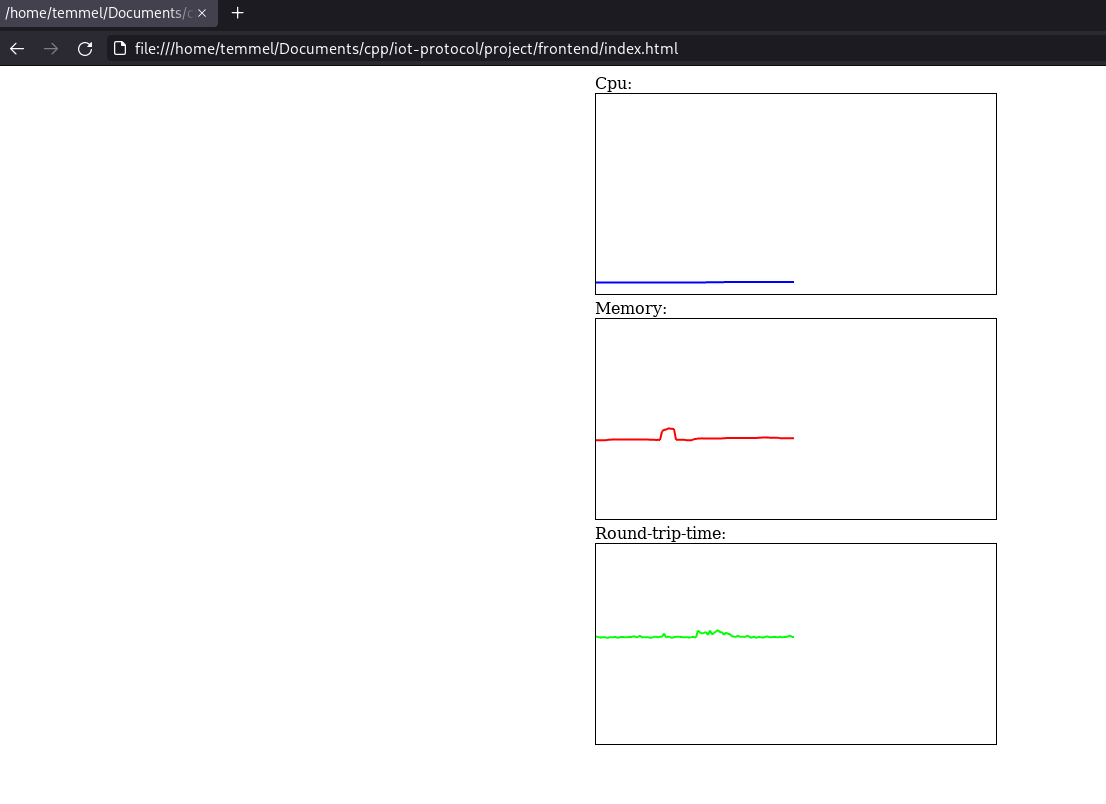
\includegraphics[width=\textwidth]{./img/stonks_graph.png}
		\caption{Screenshot showcasing the appearance of the frontend.}
		\label{final-screenshot}
	\end{center}
\end{figure}

\textit{Figure~\ref{final-screenshot}} showcases a screenshot of the resulting frontend. Three graphs are present in this screenshot, one for the CPU usage, one for the memory usage and one for the round-trip-times collected when gathering this data. The CPU and memory graphs are normalized from a scale of 0 to 100, meaning that the roof of the graph indicates 100\% usage, whereas the bottom of the graph indicates 0\% usage. The round-trip-time was treated a bit differently, with the middle of the graph being 0 milliseconds. The graph line is placed one pixel upwards for each millisecond measured as round-trip-time. 

As these measurements are rather difficult to study in detail, the website also logs each individual message to the console. In doing so, one can later reconstruct a mean value for the round-trip-time. The mean value during this run was measured to be $7.572$ milliseconds, with a standard deviation of $1.67248126$ milliseconds. These values were extracted from debug builds of all components, minus the frontend.

\iffalse
The results chapter is included when you have produced a systematic study, i.e. an evaluation of a program that you have developed, which is required for C - and D-level diploma work. In the results chapter objective results of the empirical study are presented. Keep in mind that possible comments in this chapter should only be used for clarification. Your own views and subjective (personal) comments belong in the chapter conclusion/discussion.

Strive to present the results, for example measurement-, calculations- and/or the simulation result, in a form that is as lucid and easily understandable as possible. The results are preferably presented in diagrams or tables. Accounts of interviews can be summarised, but may include concrete examples supporting your work.

Extensive results, for example complete summaries of survey results, large tables and long mathematical deductions, are placed in the appendices.
\fi
